
\begin{frame}{viruses and executable formats}
\begin{tikzpicture}
\tikzset{
    mybox/.style={draw,rectangle,minimum width=10cm,fill=white},
}
\node[mybox] (header) {
    \textbf{header}: machine type, file type, etc.
};
\node[mybox,below=0mm of header,align=center] (pHeader) {
    \textbf{program header}: ``\myemph{segments}'' to load \\
        (also, some other information) \\
    \only<2-3>{\myemph{\textbf{length edited by virus}}}
    \only<4-6>{\myemph{\textbf{new segment added by virus}}}
};
\node[mybox,below=0mm of pHeader,align=center] (seg1) {
    \textbf{segment 1 data}
};
\node[mybox,below=0mm of seg1,align=center] (seg2) {
    \textbf{segment 2 data} \\
    \only<2-3>{\myemph{\textbf{virus code + new entry point?}}}
};
\node[mybox,visible on=<4-6>,below=0mm of seg2,align=center] (seg3) {
    \myemph{\textbf{segment 3 data --- virus segment}}
};
\coordinate (annotate) at ([yshift=-1.5cm]seg2.south);
\tikzset{
    annoBox/.style={draw=red,thick,at=(annotate),font=\small,align=center},
}
\begin{visibleenv}<3,5>
    \node[annoBox] {heuristic 1: is entry point in last segment? \\ (segment usually not code)};
\end{visibleenv}
\begin{visibleenv}<6>
    \node[annoBox] {heuristic 2: did virus mess up header? \\ (e.g. do sizes used by linker but not loader disagree)
                \\ section names disagree with usage?};
\end{visibleenv}
\end{tikzpicture}
\end{frame}

\begin{frame}{defeating entry point checking}
    \begin{itemize}
    \item \myemph<2>{insert jump in normal code section, set as entry-point}
    \item add code to first section instead (perhaps insert new section at beginning)
    \end{itemize}
\begin{tikzpicture}
\tikzset{
    annoBox/.style={draw=red,thick,align=center},
}
    \begin{visibleenv}<2>
    \node[annoBox] {
        ``dynamic'' heuristic: run code in VM, see if switches sections
    };
    \end{visibleenv}
\end{tikzpicture}
\end{frame}

\begin{frame}{heuristics: library calls}
    \begin{itemize}
    \item dynamic linking --- functions called \myemph{by name}
    \item how do viruses add to dynamic linking tables?
        \begin{itemize}
        \item often don't! --- instead dynamically look-up functions
        \item if do --- could mess that up/lots of code
        \end{itemize}
    \end{itemize}

    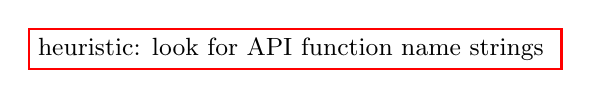
\begin{tikzpicture}
\tikzset{
    annoBox/.style={draw=red,thick,font=\small,align=center},
}
    \node[annoBox] {
        heuristic: look for API function name strings
    };
    \end{tikzpicture}
\end{frame}

\begin{frame}{evading library call checking}
    \begin{itemize}
    \item modify dynamic linking tables
        \begin{itemize}
        \item probably tricky to add new entry
        \end{itemize}
    \item reimplement library call manually
        \begin{itemize}
        \item Windows system calls not well documented, change
        \end{itemize}
    \item \myemph<2>{hide names}
    \end{itemize}
\end{frame}

\begin{frame}{hiding library call names}
    \begin{itemize}
    \item common approach: store \myemph{hash of name}
    \item runtime: read library, scan list of functions for name
    \vspace{.5cm}
    \item bonus: makes analysis harder
    \end{itemize}
\end{frame}


